\section{Synthesis}
\begin{figure}
	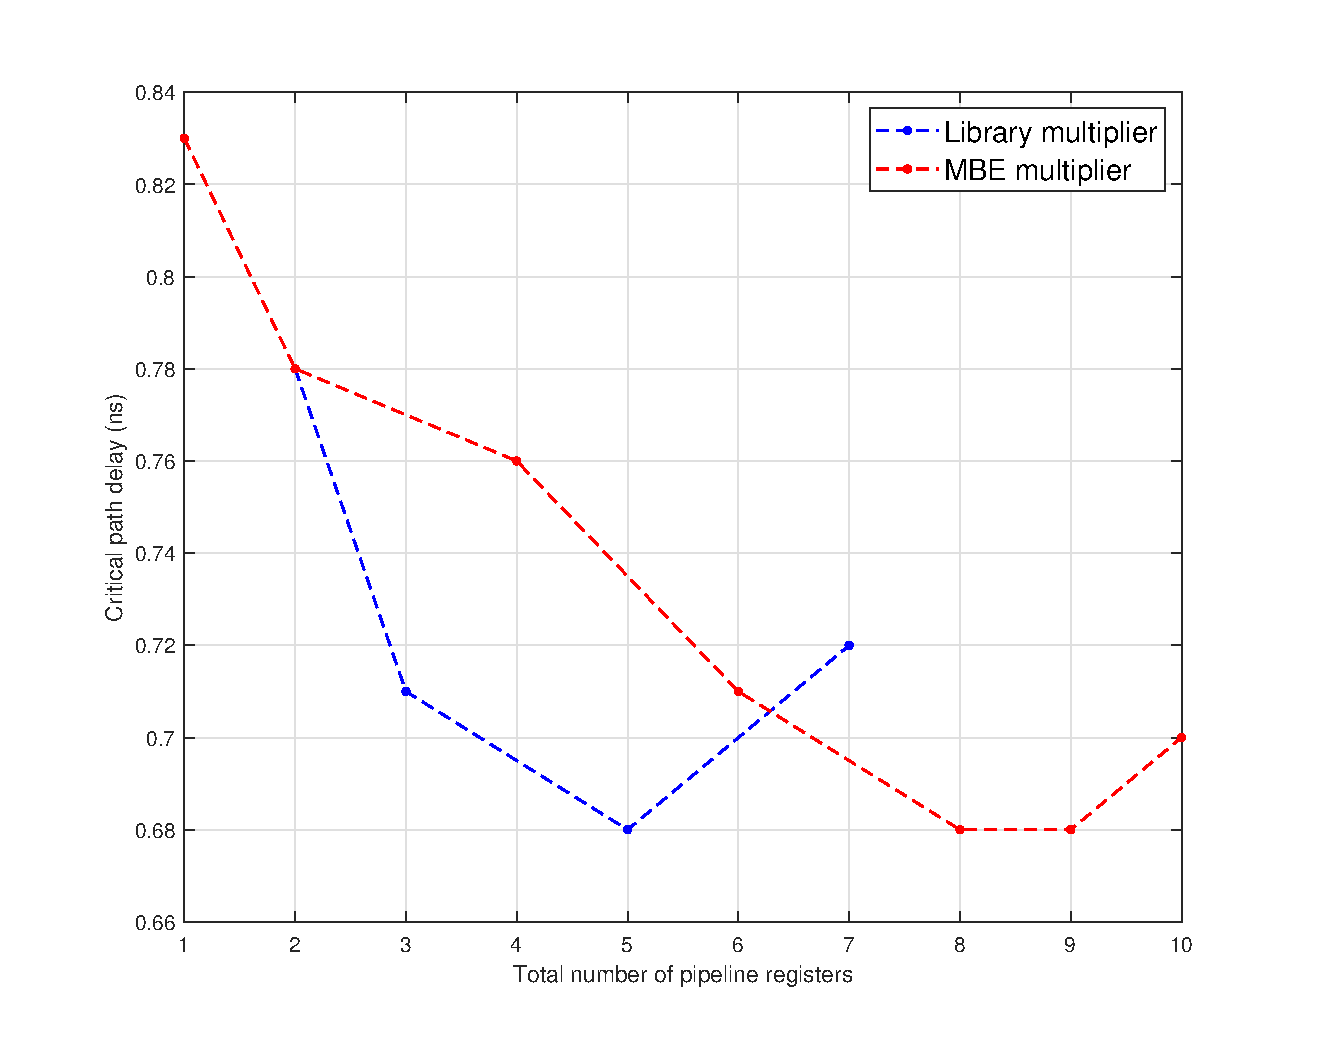
\includegraphics[width=\textwidth]{chapter2/images/delays.eps}
	\caption{Critical path delays as a function of total number of pipeline registers}
	\label{fig:delays}
\end{figure}
This new multiplier replaces the library multiplier instantiated in the second stage of \texttt{fpmul}. In order to fairly assess the impact that this component has on performance, pipeline registers are included and the synthesis process is repeated with several values of \texttt{NPIPE}, the constant denoting the number of pipeline registers.
\begin{table}
\begin{tabular}{|l|l|l|l|l|l|l|}\hline
	& No retiming & \texttt{NPIPE=1} & \texttt{NPIPE=2} & \texttt{NPIPE=4} & \texttt{NPIPE=6} & \texttt{NPIPE=8}\\\hline
	Clock period & 1.44$\,\textrm{ns}$ & 0.83$\,\textrm{ns}$& 0.78$\,\textrm{ns}$& 0.76$\,\textrm{ns}$ & 0.71 $\,\textrm{ns}$& 0.68$\,\textrm{ns}$ \\\hline
	Area (total) & 5935 & 6926 & 7130 & 7992 & 8402 & 8273 \\\hline
	Area (combinational) & 4794 & 4842 & 4655 & 4749 & 4729 & 4657 \\\hline
	Area (\texttt{mbe\_mult/add\_1424}) & 372 (6.3 \%)  & 419 (6 \%)  &  705 (9.9 \%)& 654 (8.2 \%) & 648 (7.7 \%) & 643 (7.8 \%)\\\hline
\end{tabular}
\caption{Characterization of the MBE multiplier}
\label{tab:MBE}
\end{table}
\autoref{fig:delays} shows that the MBE multiplier can potentially reach the same critical path delay as the library one, provided that more pipeline stages are inserted. This plot shows that there is an optimum number of pipeline stages, beyond which it is no longer possible to break critical paths using this technique. The MBE design reaches the minimum critical path delay with eight registers, whereas four stages are the best choice when resorting to the DesignWare component. Designs that include the MBE multiplier have been synthesized using a larger total area, as apparent by comparing \autoref{tab:MBE} with \autoref{tab:stage2}.
